\documentclass[12pt]{article}
\usepackage[slovene]{babel}
\usepackage[utf8]{inputenc}
\usepackage[T2A]{fontenc}
\usepackage{amsmath}
\usepackage{amsfonts}
\usepackage{amssymb}
\usepackage[version=4]{mhchem}
\usepackage{stmaryrd}
\usepackage{graphicx}
\usepackage[export]{adjustbox}
\graphicspath{ {./images/} }
\usepackage{physics}
\usepackage{geometry}
\geometry{left=2cm,right=2cm,top=2cm,bottom=2cm}

\title{\textbf{Določanje Boltzmannove konstante}}
\author{Samo Krejan}
\date{maj 2025}

\begin{document}
\maketitle

\section{Uvod}

Boltzmanova konstanta $k_b$ je ena izmed najpomembnejših konstant v fiziki. Mi smo jo določali na podlagi diskusije o tokovih znotraj bipolarnega tranzistorja $(n-p-n)$. To so najbolj osnovni tranzistorji sestavljeni iz dveh $p-n$ stikov.

Naš bipolarni tranzistor ima tri kontakte imenovane kolektor, emitor in baza. V vaji kolektor in bazo kratko sklenemo in merimo kolektorski tok $I_c$ v odvisnosti od napetosti med bazo in emitorjem $U_{BE}$. Tevretična napoved te odvisnosti je podana z Ebbers-Mollovo enačbo:

\begin{equation*}
    I_c(T) = I_s(T)\left[\exp(\frac{e_0U_{BE}}{k_bT}) - 1\right],
\end{equation*}
kjer je $e_0$ osnovni naboj, $T$ temperatura in $I_s(T)$ velikost nasičenega toka v zaporni smeri.

Ker že v naprej vemo, da je Boltzmannova konstanta izredno majhna, vemo, da bo eksponent izredno velik in lahko \textit{pozabimo} na $-1$ saj je efektivna napaka zaradi tega manjša od procenta. Tako dobimo poenostavljeno enačbo \ref{ebermol}:

\begin{equation}
    I_c(T) = I_s(T)\exp(\frac{e_0U_{BE}}{k_bT}),
    \label{ebermol}
\end{equation}

Pri eksperimentu smo nadzorovali napetost med bazo in emitorjem s pomočjo baterije in variabilnega upora glej vezje \ref{vezje}, temperaturo pa smo nadzorovali s pomočjo Dewarjeve posode z vodo.

\begin{figure}[ht]
\begin{center}
    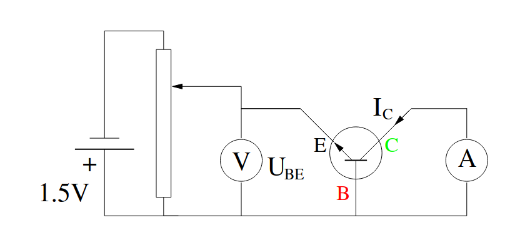
\includegraphics[width=10cm]{vezje.png}
    \caption{Skica vezja, uporabljenega skozi celotno vajo (vir: navodila)}
    \label{vezje}
\end{center}
\end{figure}


\section{Potrebščine}

\begin{itemize}
    \item bipolarni n-p-n tranzistor tipa BC182B,
    \item potenciometer in baterija (1,5 V),
    \item multimeter (Voltcraft 870) in namizni multimeter (SigLent SDM 3065X), žice,
    \item termometer, Dewarjeva posoda, grelec vode in izdelovalec ledu,
    \item prenosnik z ustrezno programsko opremo.
\end{itemize}

\section{Naloga}

\begin{enumerate}
    \item Izmerite odvisnost kolektorskega toka $I_c$ v odvisnosti od napetosti $U_{BE}$ pri temperaturah: 15, 35 in 55 stopinj,
    \item določite razmerje $e_0/k_b$,
    \item izmerite temperaturno odvisnost kolektorskega toka tranzistorja od temperature pri napetostih $U_{BE}$: 0,5 in 0,58 volta.
\end{enumerate}


\section{Rezultati in analiza}

Najprej smo merili odvisnost kolektorskega toka $I_c$ od napetosti med bazo in emitorjem $U_{BE}$. Iz enačbe \ref{ebermol} vidimo, da bi bilo koristno enačbo linearizirati z logaritmom, da bomo lahko določali razmerje $e_0/k_b$. To storimo za meritve pri vseh treh različnih temperaturah. Tako je nastal graf \ref{linbin}, ki prikazuje linearizirane vse tri meritve posebaj.

\begin{figure}[ht]
\begin{center}
    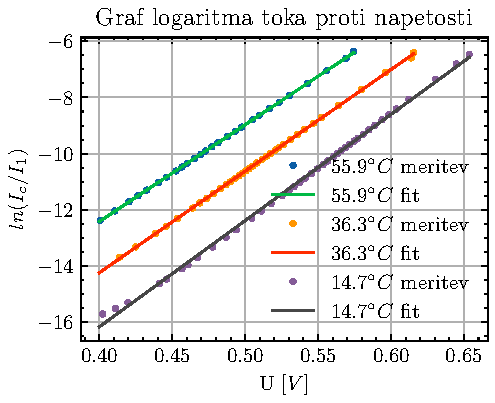
\includegraphics[width=10cm]{moju_lin.pdf}
    \caption{Linearizirane odvisnosti kolektorskega toka od napetosti}
    \label{linbin}
\end{center}
\end{figure}

\newpage
\noindent S pythonom, smo lahko zelo zanesljivo določili naklon premic na grafu \ref{linbin} s čimer smo dobili $\frac{e_0}{k_bT}$. Ko to vrednost končno pomnožimo še s temperaturo pri kateri smo izvedli posamezno meritev dobimo iskano razmerje $\frac{e_0}{k_b}$. Vrednosti so zapisane v tabeli \ref{tabela}:

\begin{table}[!ht]
\centering
\begin{tabular}{c|c}
    T [$^{\circ} C$] & $\frac{e_0}{k_b}$ [K/V] \\ \hline
    $55,9 \pm 0,6$ & $11340\pm 20$ \\
    $36,3\pm 0,3$ & $11190\pm 10$\\
    $14,7\pm 0,1$ & $10888\pm 4$\\\hline \hline
    average & $11100\pm 200$\\
\end{tabular}
\caption{preračunane vrednosti za iskano razmerje ter njegova povprečna vrednost}
\label{tabela}
\end{table}

S tem smo na žalost nekoliko zgrašili vrednost iz literature ($11604\ K/V$). A pogumno je delati statistične zaključke po treh meritvah, zato sem si sposodil še 38 meritev mojih sošolcev, kjer sem preko enakega postopka prišel do rezultata:

\begin{equation*}
    \frac{e_0}{k_b} = (11200\pm 400) K/V,
\end{equation*}
ki se dejansko strinja z teoretično vrednostjo v okviru napake.

\bigskip

\noindent Sledi raziskava odvisnosti kolektorskega toka od temperature. Merili smo pri dveh različnih napetostih $U_{BE}$ in dobili naslednje grafe \ref{iodt}:

\begin{figure}[h!]
\centering
\begin{minipage}[t]{0.45\textwidth}
    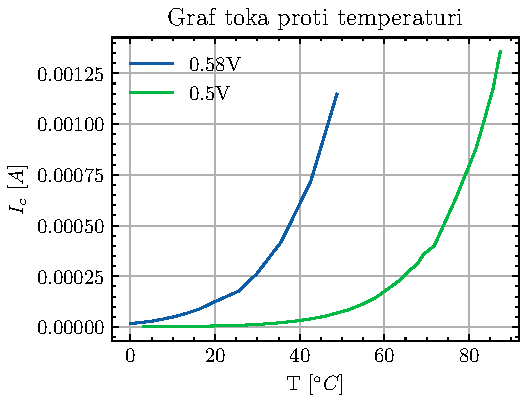
\includegraphics[width=\textwidth]{iodt.pdf}

\end{minipage}
\hfill
\begin{minipage}[t]{0.45\textwidth}
    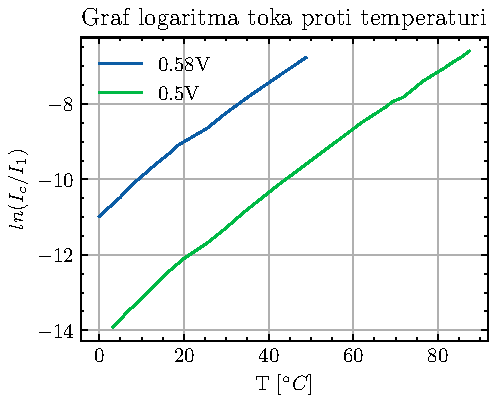
\includegraphics[width=\textwidth]{lniodt.pdf}

\end{minipage}
\caption{Meritev kolektorskega toka na levi in njegovega logaritma na desni, v odvisnosti od temperature}
\label{iodt}
\end{figure}

Kot vidimo, je odvisnost blizu eksponentni, a ne popolnoma. Kot nas navodila podučijo, nas tukaj bolj zanima neposredna meritev saturacijskega toka v odvisnosti od temperature. Slednjega lahko izrazimo iz enačbe \ref{ebermol} in odvisnost tudi grafiramo. Na ta način dobimo slednja grafa \ref{is}:

\begin{figure}[ht]
    \centering
    \begin{minipage}[t]{0.42\textwidth}
        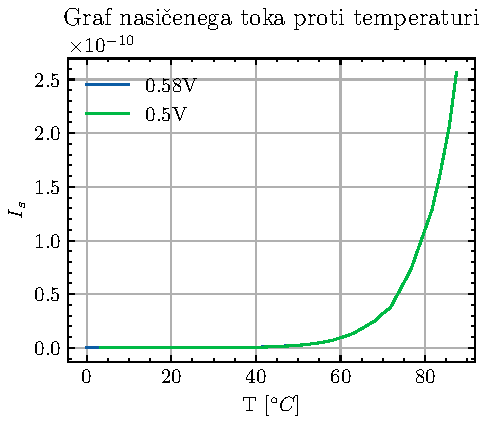
\includegraphics[width=\textwidth]{isodt.pdf}
    
    \end{minipage}
    \hfill
    \begin{minipage}[t]{0.48\textwidth}
        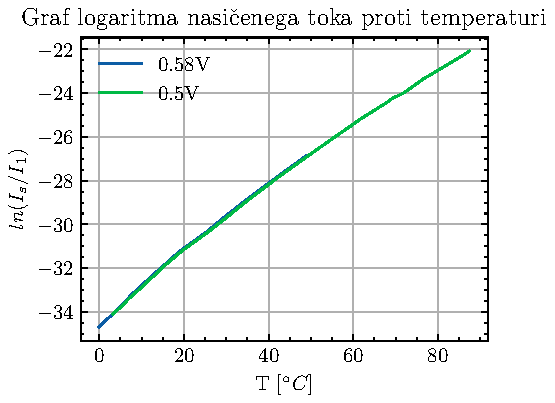
\includegraphics[width=\textwidth]{lnisodt.pdf}
    
    \end{minipage}
    \caption{Preračunane vrednosti nasičenega toka in njegovega logaritma}
    \label{is}
\end{figure}
\newpage

Nažalost mi ni uspelo na neposredno meritve nasičenega toka fitati v navodilih predstavljenega modela, a že iz slike nas ni težko prepričati, da odvisnost velja. Da smo naredili nekaj prav še bolje dokazuje dejstvo, da se grafa čez skupno definicijsko območje zelo natančno prekrivata. To dvoje skupaj nam da nekaj zaupanja, da smo res uspešno izmerili nasičen tok.


\end{document}